\documentclass[[12pt,twoside]{book}
\usepackage{_my_document_style}
\begin{document}
\begin{figure}[t]%[H]%[!htbp]
\centering
%\checkoddpage
%\centering
   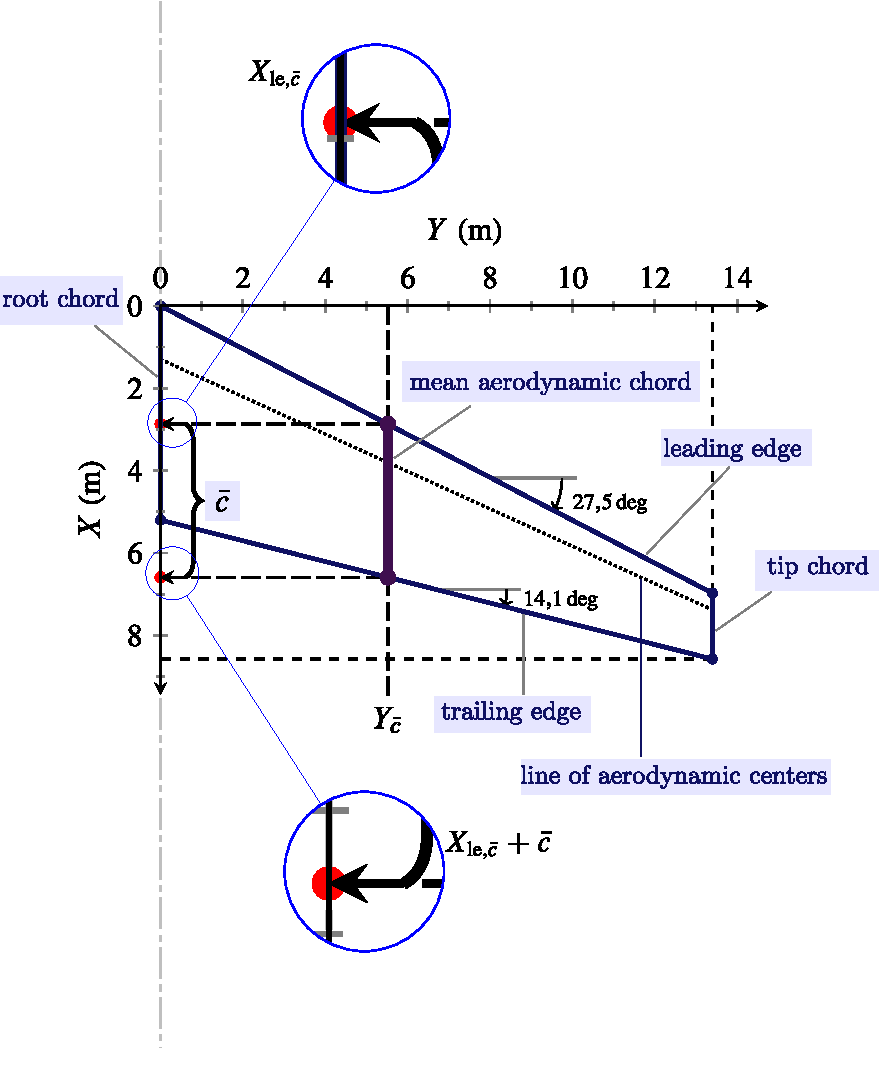
\includegraphics[width=0.78\textwidth]{Chapter_2/geometric_characteristics_of_a_wing_with_arrow_not_null/wing_planform_basic_1_drawing.pdf}%
  \caption{\finalhyphendemerits=1000
            Planform of the wing assigned in the example~\ref{example:Geometric:Characteristics:Of:A:Wing:With:Sweep:Angle:Not:Null}.}
\label{fig:Wing:Planform:Results:A}%
\end{figure}
%
\def\mySpanWingMT{26.800000}
\def\myChordRootWingMT{5.200000}
\def\myChordTipWingMT{1.600000}
\def\myTaperRatioWing{0.307692}
\def\myAreaWingMTsquared{91.120000}
\def\myMACWingMT{3.717647}
\def\myYMACWingMT{5.517647}
\def\myXLEMACWingMT{2.872305}
\def\myLambdaCQuarterDeg{24.405918}
\def\myLambdaCQuarterRad{0.425964}
\def\myLambdaCHalfDeg{21.152565}
\def\myLambdaCHalfRad{0.369182}
\def\myLambdaTEDeg{14.212850}
\def\myLambdaTERad{0.248061}
\def\myLambdaLEDeg{27.500000}
\def\myLambdaLERad{0.479966}
\def\myAspectRatioWing{7.882353}
\def\myCoefficientA{-0.268657}
\def\myCoefficientB{5.200000}

%
\begin{myExampleX}{Geometric characteristics of a wing with sweep angle not null}{\ding{46}}% \ \Keyboard\ %
\label{example:Geometric:Characteristics:Of:A:Wing:With:Sweep:Angle:Not:Null}
\noindent
The wing of an aircraft has straight leading and trailing edges, wingspan $b=\SI[round-precision=1]{\mySpanWingMT}{\metre}$,
root chord $c_\mathrm{r}=\SI[round-precision=2]{\myChordRootWingMT}{\metre}$, tip chord $c_\mathrm{t}=\SI[round-precision=2]{\myChordTipWingMT}{\metre}$
and leading edge sweep angle $\Lambda_\mathrm{le}=\SI[round-precision=1]{\myLambdaLEDeg}{\degree}$.
We want to calculate the following quantities:

\adjustbox{center=\textwidth}{%
$S$\,, $\AR$\,, $\Lambda_{c/4}$\,, $\Lambda_{c/2}$\,, $\Lambda_\mathrm{te}$\,, 
$\bar{c}$\,, $X_{\mathrm{le},\bar{c}}$\,, $Y_{\bar{c}}$
}% \,, $Y_{\bar{c}}$
\medskip

The linear law applied to section chords is:
$c \big( Y \big) = A_c \, Y + B_c$ 
where
\[
A_c
  = \frac{c_\mathrm{t} - c_\mathrm{r}}{b/2}
  = 
    2 \frac{
      \SI[round-precision=2]{\myChordTipWingMT}{\metre} - \SI[round-precision=2]{\myChordRootWingMT}{\metre}
    }{
      \SI[round-precision=2]{\mySpanWingMT}{\metre}
    }
  = \SI[round-precision=3]{\myCoefficientA}{} 
\]
\[
B_c
  = c_\mathrm{r}
  =  \SI[round-precision=2]{\myCoefficientB}{\metre} 
\]
Therefore we have
\[
c \big( Y \big) = A_c \, Y + B_c
  = \SI[round-precision=3]{\myCoefficientA}{} \, Y
    + \SI[round-precision=2]{\myCoefficientB}{\metre}
\]
The taper ratio is
\[
\lambda
  =\frac{c_\mathrm{t}}{c_\mathrm{r}}
  =\frac{\SI[round-precision=2]{\myChordTipWingMT}{\metre}}{\SI[round-precision=2]{\myAreaWingMTsquared}{\metre}}
  =\SI[round-precision=2]{\myTaperRatioWing}{} 
\]
and the wing area is
\[
\begin{split}
S & {}= \frac{b}{2} \, c_\mathrm{r} \, \big( 1 + \lambda \big) \\
  & {}=
    \num{0.5} \cdot \SI[round-precision=1]{\mySpanWingMT}{\metre}
      \cdot \SI[round-precision=2]{\myChordRootWingMT}{\metre}
      \cdot \big( 1 + \SI[round-precision=2]{\myTaperRatioWing}{} \big) 
    = \SI[round-precision=1]{\myAreaWingMTsquared}{\metre^2} 
\end{split}
\]
so we have a wing aspect ratio
\[
\AR
  = \frac{b^2}{S}
  = \frac{\big(\SI[round-precision=1]{\mySpanWingMT}{\metre}\big)^2}{\SI[round-precision=1]{\myAreaWingMTsquared}{\metre^2}}
  = \num[round-precision=2]{\myAspectRatioWing} 
\]
For the relation
\[
\tan\Lambda_{c/n} = \tan\Lambda_\mathrm{le}-\dfrac{(4/n)(1-\lambda)}{\AR(1+\lambda)}
\]
which connects the sweep angle of the leading edge $\Lambda_\mathrm{le}$  to the sweep angle $\Lambda_{c/n}$ of the line joining the points along the single chords $c(Y)$ distant $c(Y)/n$ from the local leading edge, we have
\[
\tan
\Lambda_{c/4}
   = \tan (\SI[round-precision=3]{\myLambdaLERad}{\radian})
      - \dfrac{
         \num[round-precision=2]{1.0}
         \cdot (1-\SI[round-precision=2]{\myTaperRatioWing}{})
      }{
         \num[round-precision=2]{\myAspectRatioWing}
         \cdot (1+\SI[round-precision=2]{\myTaperRatioWing}{})} 
   \quad
   \Rightarrow
   \quad
   \Lambda_{c/4}
      =\SI[round-precision=3]{\myLambdaCQuarterRad}{\radian} 
      =\SI[round-precision=1]{\myLambdaCQuarterDeg}{\deg}
\]
%
\[
\tan
\Lambda_{c/2}
   = \tan (\SI[round-precision=3]{\myLambdaLERad}{\radian})
      - \dfrac{
         \num[round-precision=2]{2.0}
         \cdot (1-\SI[round-precision=2]{\myTaperRatioWing}{})
      }{
         \num[round-precision=2]{\myAspectRatioWing}
         \cdot (1+\SI[round-precision=2]{\myTaperRatioWing}{})} 
   \quad
   \Rightarrow
   \quad
   \Lambda_{c/2}
      =\SI[round-precision=3]{\myLambdaCHalfRad}{\radian} 
      =\SI[round-precision=1]{\myLambdaCHalfDeg}{\deg} 
\]
%
\[
\tan
\Lambda_\mathrm{te}
   = \tan (\SI[round-precision=3]{\myLambdaLERad}{\radian})
      - \dfrac{
         \num[round-precision=2]{4.0}
         \cdot (1-\SI[round-precision=2]{\myTaperRatioWing}{})
      }{
         \num[round-precision=2]{\myAspectRatioWing}
         \cdot (1+\SI[round-precision=2]{\myTaperRatioWing}{})} 
   \quad
   \Rightarrow
   \quad
   \Lambda_\mathrm{te}
      =\SI[round-precision=3]{\myLambdaTERad}{\radian}
      =\SI[round-precision=1]{\myLambdaTEDeg}{\deg} 
\]
It is observed that the characteristic sweep angles of the shape in plan go progressively decreasing passing from the leading edge ($\Lambda_\mathrm{le}$), 
to the quarter chord line ($\Lambda_{c/4}$),
to the midline ($\Lambda_{c/2}$),
to the trailing edge ($\Lambda_\mathrm{te}$).
The value of the mean aerodynamic chord is the following:
\[
\begin{split}
\bar{c} & {}= \frac{2}{3} \, c_\mathrm{r} \, \frac{1+\lambda + \lambda^2}{1+\lambda} \\
  & {}=
    \num{0.667} \cdot \SI[round-precision=2]{\myChordRootWingMT}{\metre}
      \cdot 
        \frac{
          1 + \SI[round-precision=2]{\myTaperRatioWing}{} + \SI[round-precision=2]{\myTaperRatioWing}{}^2
        }{
          1 + \SI[round-precision=2]{\myTaperRatioWing}{}
        }
    = \SI[round-precision=2]{\myMACWingMT}{\metre} 
\end{split}
\]
The longitudinal distance of the mean aerodynamic chord's leading edge from the leading edge of the root chord is:
\[
\begin{split}
X_{\mathrm{le},\bar{c}} 
  & {}=
    \frac{b}{6} \, \frac{1+2\lambda}{1+\lambda} \tan\Lambda_\mathrm{le} \\[3pt]
  & {}=
    \frac{\SI[round-precision=1]{\mySpanWingMT}{\metre}}{6}
      \cdot 
      \frac{
        1 + 2\cdot\SI[round-precision=2]{\myTaperRatioWing}{}
      }{
        1 + \SI[round-precision=2]{\myTaperRatioWing}{}
      }
      \cdot \tan \big( \SI[round-precision=3]{\myLambdaLERad}{\radian} \big)
    = \SI[round-precision=2]{\myXLEMACWingMT}{\metre} 
\end{split}
\]
It is observed that for a tapered wing with sweep angle not null, there is a
$X_{\mathrm{le},\bar{c}}$ not null. This means that the projection of the wing section having chord equal to $\bar{c}$ in the middle plane is further back than the root chord.
Also, given the value of $\bar{c}$ previously calculated, this projection
is not entirely internal to the root chord but has an abscissa of trailing edge $X_{\mathrm{le},\bar{c}}+\bar{c}>c_\mathrm{r}$.
The station $Y_{\bar{c}}$ to which the law of the chords $c(Y)$ assumes valuev$\bar{c}$ is:
\[
\begin{split}
Y_{\bar{c}} 
  & {}=
    \frac{b}{6} \, \frac{1+2\lambda}{1+\lambda} \\[3pt]
  & {}=
    \frac{\SI[round-precision=1]{\mySpanWingMT}{\metre}}{6}
      \cdot 
      \frac{
        1 + 2\cdot\SI[round-precision=2]{\myTaperRatioWing}{}
      }{
        1 + \SI[round-precision=2]{\myTaperRatioWing}{}
      }
    =  \SI[round-precision=2]{\myYMACWingMT}{\metre} 
\end{split}
\]
% \begin{figure}[t]
%     \centering
%     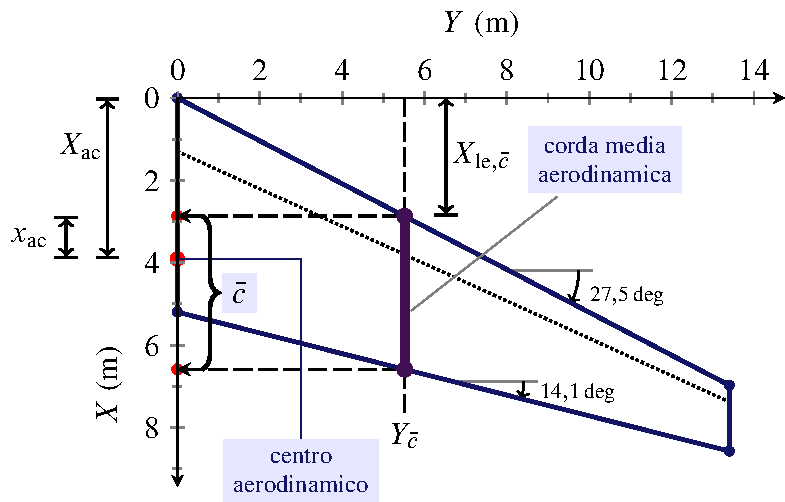
\includegraphics[width=0.8\textwidth]{Chapter_2/temp/wing_ac_1_drawing.pdf}
%     \rule{2cm}{0pt}
%     \caption{Insert caption here}
%     \label{fig:my:label}
% \end{figure}
The point of coordinates $(X_{\mathrm{le},\bar{c}},0)$ is of extreme importance in the formulation of the pitch equilibrium equations and of the static stability condition at aircraft pitching. This point is taken as a reference by the designers for evaluating the position of the center of gravity and the characteristic aerodynamic centers of the aircraft
(of the isolated wing, of the wing-fuselage configuration, of the complete aircraft). For example, if a given characteristic point $P$ has a longitudinal distance $a\bar{c}$ from the leading edge of mean aerodynamic chord with $a$ dimensionless), a coordinate is introduced $x$ such that $x_P = X_P - X_{\mathrm{le},\bar{c}} = a\bar{c}$. It is also said that the dimensionless position of $P$ compared to the leading edge of the mean
aerodynamic chord is $\bar{x}_P=a$.
\end{myExampleX}
\end{document} 
